\documentclass{standalone}
\usepackage{tikz,pgfplots}
\pgfplotsset{compat=1.18}
\begin{document}
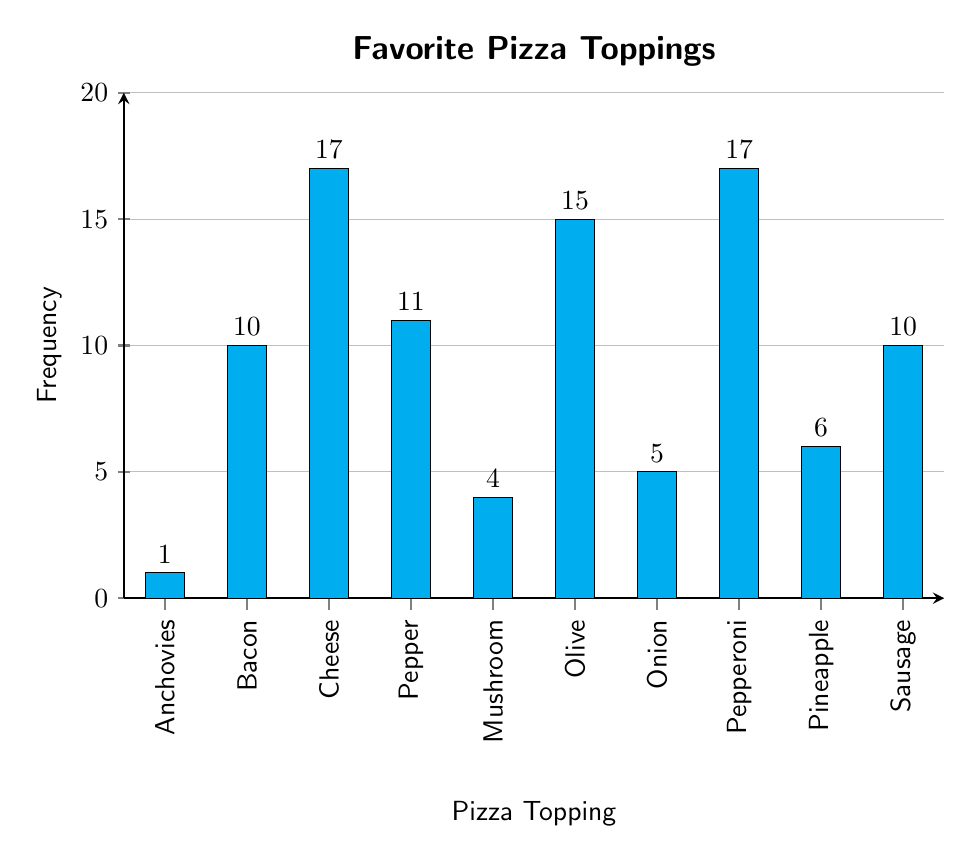
\begin{tikzpicture}[font=\sffamily] % Apply \sffamily to the entire picture
\begin{axis}[
    axis lines=left,
    no markers,
    xmin = 0.5, xmax=10.5,
    ymin=0, ymax=20,
    xtick={1,2,3,4,5,6,7,8,9,10},
    ytick={0,5,10,15,20},
    xticklabels={Anchovies,Bacon,Cheese,Pepper,Mushroom,Olive,Onion,Pepperoni,Pineapple,Sausage},
    ticklabel style={font=\normalsize\sffamily},
    xticklabel style={rotate=90},
    xlabel style={font=\sffamily, yshift=-0.5cm},
    xlabel={Pizza Topping},
    ylabel style={font=\sffamily},
    ylabel={Frequency},
    title={Favorite Pizza Toppings},
    title style={font=\large\sffamily\bfseries},
    enlargelimits=false,
    clip=false,
    grid = none,
    ymajorgrids=true,
    ybar=0pt,
    bar width=.5cm,
    width=12cm,
    height=8cm,
    axis line style={thick},
    tick style={thick},
]
\addplot[fill=cyan, draw=black] coordinates {
    (1,1)   % Anchovies
    (2,10)  % Bacon
    (3,17)  % Cheese
    (4,11)  % Pepper
    (5,4)   % Mushroom
    (6,15)  % Olive
    (7,5)   % Onion
    (8,17)  % Pepperoni
    (9,6)   % Pineapple
    (10,10) % Sausage
};

% Add value labels on top of bars
\addplot[
    nodes near coords,
    nodes near coords style={font=\normalsize\sffamily, anchor=south},
    only marks,
    mark=none
] coordinates {
    (1,1) (2,10) (3,17) (4,11) (5,4) (6,15) (7,5) (8,17) (9,6) (10,10)
};

\end{axis}
\end{tikzpicture}
\end{document}
